\documentclass[12pt]{article}

% PACKAGES
\usepackage{amsmath, amssymb}   % For math symbols and environments
\usepackage{graphicx}           % For including images
\usepackage{fancyhdr}           % For headers and footers
\usepackage{hyperref}           % For clickable references
\usepackage{geometry}           % For page margins
\usepackage{color}              % For color text
\usepackage{listings}           % For code listings
\usepackage{caption}            % For customizing figure and table captions
\usepackage{float}              % For floating figures and tables
\usepackage{tcolorbox}          % For boxed notes or highlights

% FONTS
\usepackage[T1]{fontenc}
\usepackage[utf8]{inputenc}
\usepackage{newpxtext,newpxmath}
\usepackage{sectsty}

% PAGE LAYOUT
\geometry{
	a4paper,
	left=25mm,
	right=25mm,
	top=25mm,
	bottom=25mm
}

% HEADER AND FOOTER SETTINGS
\pagestyle{fancy}
\fancyhf{}
\fancyhead[L]{Lecture Notes: Module-Lattice-Based Key-Encapsulation Mechanism}
\fancyhead[R]{\thepage}

% CODE LISTINGS STYLE FOR *.c FILES
\lstset{
	frame=tb,
	language=C,
	aboveskip=3mm,
	belowskip=3mm,
	showstringspaces=false,
	columns=flexible,
	basicstyle={\small\ttfamily},
	numbers=left,
	numberstyle=\tiny\color{gray},
	keywordstyle=\color{blue},
	commentstyle=\color{green},
	stringstyle=\color{red},
	breaklines=true,
	breakatwhitespace=true,
	tabsize=4,
	captionpos=b
}

% HYPERLINK COLORS
\hypersetup{
	colorlinks=true,
	linkcolor=blue,
	citecolor=green,
	filecolor=magenta,
	urlcolor=cyan,
}

% TIKZPTICTURES
\usepackage{algorithm}
\usepackage{algorithmic}
\usepackage{tikz}
\usepackage{geometry}


\newtheorem{definition}{Definition}
\newtheorem{theorem}{Theorem}
\newtheorem{example}{Example}
\newtheorem{remark}{Remark}
\newtheorem{observation}{Observation}

% DOCUMENT BEGINS
\begin{document}
	
	% TITLE AND AUTHOR INFO
	\title{Lecture Notes: Preliminaries of Module-Lattice-Based Key-Encapsulation Mechanism}
	\author{Ji, Yong-Hyeon}
	\date{\today}
	\maketitle
	
	\tableofcontents  % Generates the table of contents
	\newpage

	\section{Introduction}
	
	In this lecture, we will cover the preliminary concepts for understanding Module-Lattice-based Key Encapsulation Mechanisms (KEM). To make abstract concepts more accessible, each definition will be followed by several concrete examples and observations, with visualizations. This will help bridge the gap between abstract theory and intuitive understanding.
	
	\section{Linear Algebra and Euclidean Lattices}
	
	\subsection{Vectors and Vector Spaces}
	
	\begin{definition}
		A \textbf{vector space} $V$ over a field $\mathbb{F}$ is a set of vectors where two operations are defined:
		\begin{itemize}
			\item Vector addition: $\mathbf{u} + \mathbf{v}$
			\item Scalar multiplication: $c \cdot \mathbf{v}$ for $c \in \mathbb{F}$
		\end{itemize}
		The space $V$ is closed under these operations, meaning if you add two vectors or multiply a vector by a scalar, the result stays in $V$.
	\end{definition}
	
	\begin{example}
		The space $\mathbb{R}^2$ consists of vectors of the form $\mathbf{v} = (v_1, v_2)$, where $v_1, v_2 \in \mathbb{R}$. An example of vector addition in $\mathbb{R}^2$:
		\[
		(1, 2) + (3, 4) = (4, 6).
		\]
	\end{example}
	
	\begin{example}
		The space $\mathbb{R}^3$ consists of vectors like $\mathbf{v} = (v_1, v_2, v_3)$. Consider the vector $\mathbf{v} = (1, -1, 2)$ and a scalar $c = 2$. Then scalar multiplication gives:
		\[
		2 \cdot (1, -1, 2) = (2, -2, 4).
		\]
	\end{example}
	
	\begin{observation}
		Vector spaces are abstractions that generalize the familiar idea of points and lines in 2D and 3D spaces. Working with $\mathbb{R}^2$ and $\mathbb{R}^3$ as concrete examples helps ground the abstract notion of higher-dimensional vector spaces.
	\end{observation}
	
	\begin{center}
		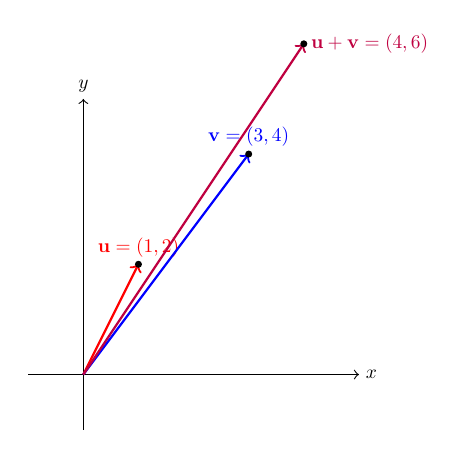
\begin{tikzpicture}[scale=0.7, transform shape]
			% Axes
			\draw[->] (-1, 0) -- (5, 0) node[right] {$x$};
			\draw[->] (0, -1) -- (0, 5) node[above] {$y$};
			
			% Vector u
			\draw[->, thick, red] (0, 0) -- (1, 2) node[above] {$\mathbf{u} = (1, 2)$};
			
			% Vector v
			\draw[->, thick, blue] (0, 0) -- (3, 4) node[above] {$\mathbf{v} = (3, 4)$};
			
			% Resultant vector
			\draw[->, thick, purple] (0, 0) -- (4, 6) node[right] {$\mathbf{u} + \mathbf{v} = (4, 6)$};
			
			% Labels
			\filldraw[black] (1, 2) circle (1.5pt) node[below right] {};
			\filldraw[black] (3, 4) circle (1.5pt) node[below right] {};
			\filldraw[black] (4, 6) circle (1.5pt) node[below right] {};
		\end{tikzpicture}
		
	\end{center}
	
	\subsection{Lattices in Vector Spaces}
	
	\begin{definition}
		A \textbf{lattice} $\Lambda$ in a vector space $\mathbb{R}^n$ is a set of points formed by all integer linear combinations of a set of linearly independent vectors, $\mathbf{b}_1, \mathbf{b}_2, \dots, \mathbf{b}_n$. 
		\[
		\Lambda = \left\{ \sum_{i=1}^n z_i \mathbf{b}_i : z_i \in \mathbb{Z} \right\}.
		\]
		Here, $\{\mathbf{b}_1, \dots, \mathbf{b}_n\}$ is called a \textbf{basis} of the lattice.
	\end{definition}
	
	\begin{example}
		In $\mathbb{R}^2$, let $\mathbf{b}_1 = (1, 0)$ and $\mathbf{b}_2 = (0, 1)$. The lattice generated by these vectors is $\mathbb{Z}^2$, which consists of all points with integer coordinates, i.e., 
		\[
		\Lambda = \{ (z_1, z_2) : z_1, z_2 \in \mathbb{Z} \}.
		\]
		For example, $(2, 3) \in \Lambda$, and $(\frac{1}{2}, 1) \notin \Lambda$.
	\end{example}
	
	\begin{example}
		Consider the vectors $\mathbf{b}_1 = (2, 0)$ and $\mathbf{b}_2 = (0, 2)$ in $\mathbb{R}^2$. The lattice generated by these vectors is a scaled version of $\mathbb{Z}^2$, consisting of points with even integer coordinates:
		\[
		\Lambda = \{ (2z_1, 2z_2) : z_1, z_2 \in \mathbb{Z} \}.
		\]
		Thus, points like $(2, 4)$ are in the lattice, but $(1, 3)$ is not.
	\end{example}
	
	\begin{observation}
		Lattices can be visualized as grids of points. The vectors used to generate the lattice define the spacing and structure of the grid. Changing the basis vectors changes the grid’s shape, but the fundamental lattice structure remains the same.
	\end{observation}
	
	\begin{center}
		\begin{tikzpicture}[scale=0.7, transform shape]
			% Axes
			\draw[->] (-1, 0) -- (6, 0) node[right] {$x$};
			\draw[->] (0, -1) -- (0, 6) node[above] {$y$};
			
			% Grid points for lattice Z^2
			\foreach \x in {-1,0,...,5} {
				\foreach \y in {-1,0,...,5} {
					\filldraw[black] (\x,\y) circle (1.5pt);
				}
			}
			
			% Basis vectors
			\draw[->, thick, red] (0, 0) -- (1, 0) node[below right] {$\mathbf{b}_1 = (1, 0)$};
			\draw[->, thick, blue] (0, 0) -- (0, 1) node[above left] {$\mathbf{b}_2 = (0, 1)$};
			
		\end{tikzpicture}
		
	\end{center}
	
	\subsection{Norms and Closest Vector Problem (CVP)}
	
	\begin{definition}
		The \textbf{Euclidean norm} of a vector $\mathbf{v} = (v_1, v_2, \dots, v_n) \in \mathbb{R}^n$ is the length of the vector, given by:
		\[
		\|\mathbf{v}\| = \sqrt{v_1^2 + v_2^2 + \cdots + v_n^2}.
		\]
	\end{definition}
	
	\begin{example}
		For the vector $\mathbf{v} = (3, 4)$ in $\mathbb{R}^2$, the Euclidean norm is:
		\[
		\|\mathbf{v}\| = \sqrt{3^2 + 4^2} = \sqrt{9 + 16} = 5.
		\]
		This is the length of the vector from the origin to the point $(3, 4)$.
	\end{example}
	
	\begin{definition}
		The \textbf{Closest Vector Problem (CVP)} asks: Given a lattice $\Lambda \subset \mathbb{R}^n$ and a target point $\mathbf{t} \in \mathbb{R}^n$, find the lattice point $\mathbf{v} \in \Lambda$ that is closest to $\mathbf{t}$ in terms of Euclidean distance.
	\end{definition}
	
	\begin{example}
		Let $\Lambda = \mathbb{Z}^2$ and the target point be $\mathbf{t} = (1.7, 3.2)$. The closest lattice point in $\Lambda$ is $(2, 3)$ because:
		\[
		\| (1.7, 3.2) - (2, 3) \| = \sqrt{(1.7 - 2)^2 + (3.2 - 3)^2} = \sqrt{0.09 + 0.04} = \sqrt{0.13}.
		\]
		This is smaller than the distance to any other lattice point.
	\end{example}
	
	\begin{observation}
		The CVP is intuitively about finding the nearest "grid point" to a given point. Although this seems easy in low dimensions (like 2D), it becomes computationally hard in high dimensions, which makes it suitable for cryptographic applications.
	\end{observation}
	
	\begin{center}
		\begin{tikzpicture}[scale=0.7, transform shape]
			% Axes
			\draw[->] (-1, 0) -- (6, 0) node[right] {$x$};
			\draw[->] (0, -1) -- (0, 6) node[above] {$y$};
			
			% Grid points for lattice Z^2
			\foreach \x in {0,1,...,5} {
				\foreach \y in {0,1,...,5} {
					\filldraw[black] (\x,\y) circle (1.5pt);
				}
			}
			
			% Target point
			\filldraw[red] (1.7, 3.2) circle (2pt) node[above] {$\mathbf{t} = (1.7, 3.2)$};
			
			% Nearest lattice point
			\draw[->, thick, purple] (1.7, 3.2) -- (2, 3);
			\filldraw[blue] (2, 3) circle (2pt) node[below right] {Closest point $(2, 3)$};
		\end{tikzpicture}
	\end{center}
	
	\section{Introduction to Modules}
	
	\subsection{Rings}
	
	\begin{definition}
		A \textbf{ring} $R$ is a set with two operations: addition and multiplication. It satisfies properties similar to the integers, including distributivity of multiplication over addition. Examples of rings include $\mathbb{Z}$ and $\mathbb{Z}_q$ (integers modulo $q$).
	\end{definition}
	
	\begin{example}
		Consider the ring $\mathbb{Z}_5 = \{0, 1, 2, 3, 4\}$. Addition and multiplication are performed modulo 5:
		\[
		2 + 4 = 1 \quad (\text{mod } 5), \quad 3 \times 4 = 2 \quad (\text{mod } 5).
		\]
	\end{example}
	
	\begin{example}
		The ring $\mathbb{Z}$ (integers) supports familiar operations:
		\[
		2 + 3 = 5, \quad 4 \times 5 = 20.
		\]
		However, $\mathbb{Z}$ has no bounds like $\mathbb{Z}_5$, which loops back when reaching 5.
	\end{example}
	
	\begin{observation}
		Rings generalize the structure of numbers under addition and multiplication. Familiar rings like integers and modular integers are foundational to many cryptographic constructions.
	\end{observation}
	
	\section{Conclusion}
	
	In this lecture, we introduced lattice and module lattice concepts, grounding them in several concrete examples and visualizations. These ideas form the foundation for Module-Lattice-based Key Encapsulation Mechanisms (KEMs), which we will explore in more detail in the following lectures.
	
	\newpage
	
	\section{Module Lattices and Cryptographic Applications}
	
	Lattice-based cryptography is an important area of post-quantum cryptography, and module lattices provide an efficient and flexible framework for building cryptographic schemes. In this section, we introduce the concept of module lattices step by step, using examples to make the abstract theory clearer and visualizations to build an intuitive understanding of these structures.
	
	\subsection{Module Lattices}
	
	\begin{definition}
		A \textbf{module lattice} is a lattice that is also a module over some ring $R$. Formally, it consists of integer linear combinations of basis vectors, but the coefficients come from the ring $R$ rather than the integers.
	\end{definition}
	
	\subsubsection{Step-by-Step Explanation}
	To understand module lattices, let’s break down the key components:
	\begin{itemize}
		\item \textbf{Lattice}: A lattice is a grid of points generated by integer combinations of basis vectors. The simplest example is the integer lattice $\mathbb{Z}^2$, which can be visualized as a regular grid of points in the plane.
		\item \textbf{Module over a ring}: A module generalizes vector spaces by allowing the coefficients (scalars) to come from a ring, rather than a field. Rings allow operations like addition and multiplication, but without requiring division.
		\item \textbf{Module Lattice}: In a module lattice, the grid-like structure of a lattice is combined with the algebraic structure of a module over a ring.
	\end{itemize}
	
	\subsection{Example 1: Module Lattice over \(\mathbb{Z}_5\)}
	
	Let’s begin with a concrete example to make this more intuitive.
	
	\begin{example}
		Consider the ring $\mathbb{Z}_5 = \{0, 1, 2, 3, 4\}$ (integers modulo 5) and the vectors $\mathbf{b}_1 = (1, 0)$, $\mathbf{b}_2 = (0, 1)$ in $\mathbb{R}^2$. The module lattice over $\mathbb{Z}_5$ is formed by taking all combinations of $\mathbf{b}_1$ and $\mathbf{b}_2$ with coefficients from $\mathbb{Z}_5$. That is:
		\[
		\Lambda = \left\{ z_1 \mathbf{b}_1 + z_2 \mathbf{b}_2 : z_1, z_2 \in \mathbb{Z}_5 \right\}.
		\]
		The points of the lattice are given by $(z_1, z_2)$ where $z_1, z_2 \in \{0, 1, 2, 3, 4\}$.
		
		For example, $(3, 4)$ is in the lattice since $z_1 = 3$ and $z_2 = 4$ are elements of $\mathbb{Z}_5$.
	\end{example}
	
	\begin{observation}
		In this example, the module lattice takes on a periodic structure because the coefficients are restricted to a finite set (modulo 5). This results in a finite number of points in the lattice, forming a grid structure within a bounded region. The periodicity of the lattice can be visualized as repeating blocks of points.
	\end{observation}
	
	\begin{center}
		\begin{tikzpicture}[scale=0.7, transform shape]
			% Axes
			\draw[->] (-1, 0) -- (6, 0) node[right] {$x$};
			\draw[->] (0, -1) -- (0, 6) node[above] {$y$};
			
			% Grid points for the module lattice over Z_5
			\foreach \x in {0,1,2,3,4} {
				\foreach \y in {0,1,2,3,4} {
					\filldraw[black] (\x,\y) circle (2pt);
				}
			}
			
			% Label example point (3, 4)
			\filldraw[red] (3,4) circle (3pt) node[above] {$(3,4) \in \Lambda$};
			
			% Basis vectors
			\draw[->, thick, blue] (0,0) -- (1,0) node[below] {$\mathbf{b}_1$};
			\draw[->, thick, blue] (0,0) -- (0,1) node[left] {$\mathbf{b}_2$};
			
			% Boundary box for the grid (modulo 5)
			\draw[dashed, thick] (0,0) rectangle (5,5);
			
		\end{tikzpicture}
	\end{center}
	
	\subsection{Example 2: Module Lattice over \(\mathbb{Z}_7\)}
	
	\begin{example}
		Now consider the ring $\mathbb{Z}_7$ (integers modulo 7) and the same basis vectors $\mathbf{b}_1 = (1, 0)$ and $\mathbf{b}_2 = (0, 1)$ in $\mathbb{R}^2$. The module lattice over $\mathbb{Z}_7$ is given by:
		\[
		\Lambda = \left\{ z_1 \mathbf{b}_1 + z_2 \mathbf{b}_2 : z_1, z_2 \in \mathbb{Z}_7 \right\}.
		\]
		The points of the lattice are given by $(z_1, z_2)$ where $z_1, z_2 \in \{0, 1, 2, 3, 4, 5, 6\}$.
		
		For example, $(5, 6)$ is in the lattice because $z_1 = 5$ and $z_2 = 6$ are elements of $\mathbb{Z}_7$.
	\end{example}
	
	\begin{observation}
		In this example, the periodicity is different because the coefficients come from $\mathbb{Z}_7$. This creates a larger, more spread-out grid of points, compared to the previous example. The concept of using different rings ($\mathbb{Z}_5$, $\mathbb{Z}_7$, etc.) allows for modular arithmetic that creates different lattice structures.
	\end{observation}
	
	\begin{center}
		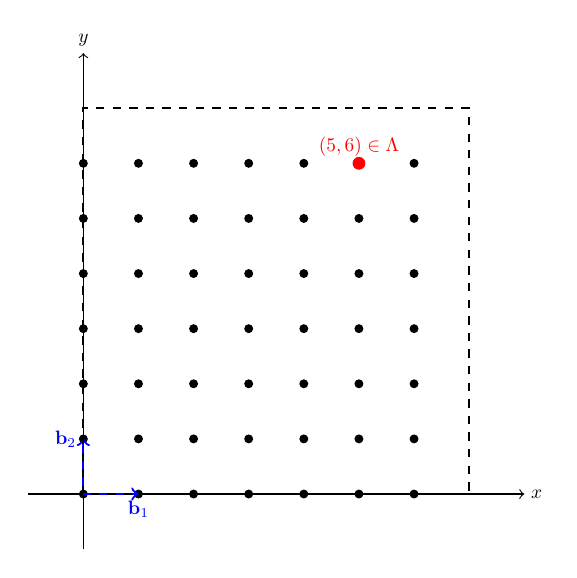
\begin{tikzpicture}[scale=0.7, transform shape]
			% Axes
			\draw[->] (-1, 0) -- (8, 0) node[right] {$x$};
			\draw[->] (0, -1) -- (0, 8) node[above] {$y$};
			
			% Grid points for the module lattice over Z_7
			\foreach \x in {0,1,2,3,4,5,6} {
				\foreach \y in {0,1,2,3,4,5,6} {
					\filldraw[black] (\x,\y) circle (2pt);
				}
			}
			
			% Label example point (5, 6)
			\filldraw[red] (5,6) circle (3pt) node[above] {$(5,6) \in \Lambda$};
			
			% Basis vectors
			\draw[->, thick, blue] (0,0) -- (1,0) node[below] {$\mathbf{b}_1$};
			\draw[->, thick, blue] (0,0) -- (0,1) node[left] {$\mathbf{b}_2$};
			
			% Boundary box for the grid (modulo 7)
			\draw[dashed, thick] (0,0) rectangle (7,7);
			
		\end{tikzpicture}
	\end{center}
	
	\subsection{Example 3: Non-Standard Basis Vectors}
	
	\begin{example}
		Let’s now change the basis vectors to something less standard. Consider the ring $\mathbb{Z}_3$ and the basis vectors $\mathbf{b}_1 = (2, 1)$ and $\mathbf{b}_2 = (-1, 2)$. The module lattice over $\mathbb{Z}_3$ is given by:
		\[
		\Lambda = \left\{ z_1 \mathbf{b}_1 + z_2 \mathbf{b}_2 : z_1, z_2 \in \mathbb{Z}_3 \right\}.
		\]
		Here, the lattice points will form a more skewed grid due to the non-standard choice of basis vectors.
		
		For example, the point $(1, 2)$ can be written as $1\mathbf{b}_1 + 2\mathbf{b}_2 = (1, 2)$.
	\end{example}
	
	\begin{observation}
		Changing the basis vectors changes the shape of the grid. Instead of forming a standard rectangular grid, the points now form a rhombus-like pattern. The flexibility in choosing basis vectors and rings allows for different lattice structures, which can be tailored to specific cryptographic applications.
	\end{observation}
	
	\begin{center}
		\begin{tikzpicture}[scale=0.7, transform shape]
			% Axes
			\draw[->] (-4, 0) -- (6, 0) node[right] {$x$};
			\draw[->] (0, -2) -- (0, 6) node[above] {$y$};
			
			% Lattice points using the non-standard basis
			\foreach \x in {-1,0,1,2} {
				\foreach \y in {-1,0,1,2} {
					\filldraw[black] (\x * 2 + \y * -1, \x * 1 + \y * 2) circle (2pt);
				}
			}
			
			% Label example point (1, 2)
			\filldraw[red] (1,2) circle (3pt) node[above] {$(1,2) \in \Lambda$};
			
			% Basis vectors
			\draw[->, thick, blue] (0,0) -- (2,1) node[below right] {$\mathbf{b}_1 = (2,1)$};
			\draw[->, thick, blue] (0,0) -- (-1,2) node[left] {$\mathbf{b}_2 = (-1,2)$};
			
		\end{tikzpicture}
	\end{center}
	
	\section{Conclusion}
	
	In this lecture, we introduced the concept of module lattices and illustrated how these structures are formed by combining lattices and modules over rings. We explored several concrete examples and visualized them using different rings and basis vectors. These examples show the flexibility of module lattices in forming different grid structures, which are essential in cryptographic constructions.
	
	
	
	
% ========================================================================================================	
% ========================================================================================================	
% ========================================================================================================	
	
%	\section{Introduction}
%	
%	In this lecture, we will cover the preliminary concepts required to understand Module-Lattice-based Key Encapsulation Mechanisms (KEM). Lattice-based cryptography is a cornerstone of post-quantum cryptography due to its security properties against quantum attacks. Our goal is to build from the basics of linear algebra and number theory to the more abstract world of lattices, modules, and their applications in cryptographic constructions.
%	
%	The approach is to first introduce concrete examples, then derive the more abstract notions from them. This way, students can intuitively grasp the essential concepts before diving into the formal definitions.
%	
%	\section{Linear Algebra and Euclidean Lattices}
%	
%	We begin with the basics of linear algebra, which forms the backbone of lattice-based cryptography.
%	
%	\subsection{Vectors and Vector Spaces}
%	
%	\begin{definition}
%		A \textbf{vector space} $V$ over a field $\mathbb{F}$ is a set of elements (called vectors) that can be added together and scaled by elements of $\mathbb{F}$. Formally, $V$ is closed under vector addition and scalar multiplication.
%	\end{definition}
%	
%	\begin{example}
%		Consider the vector space $\mathbb{R}^2$ over the field $\mathbb{R}$. Elements of $\mathbb{R}^2$ are 2-dimensional vectors, e.g., $\mathbf{v} = (v_1, v_2)$, where $v_1, v_2 \in \mathbb{R}$. Addition and scalar multiplication follow familiar rules from linear algebra:
%		\[
%		\mathbf{u} + \mathbf{v} = (u_1 + v_1, u_2 + v_2), \quad c \cdot \mathbf{v} = (c v_1, c v_2), \quad c \in \mathbb{R}.
%		\]
%	\end{example}
%	
%	\subsection{Euclidean Lattices}
%	
%	A lattice is a discrete subset of a vector space. Informally, lattices can be thought of as an infinite grid of points that repeat periodically.
%	
%	\begin{definition}
%		A \textbf{lattice} $\Lambda \subset \mathbb{R}^n$ is the set of all integer linear combinations of a set of linearly independent vectors $\mathbf{b}_1, \mathbf{b}_2, \dots, \mathbf{b}_n \in \mathbb{R}^n$. Formally, 
%		\[
%		\Lambda = \left\{ \mathbf{v} \in \mathbb{R}^n : \mathbf{v} = \sum_{i=1}^n z_i \mathbf{b}_i, \, z_i \in \mathbb{Z} \right\},
%		\]
%		where $\mathbf{B} = \{\mathbf{b}_1, \mathbf{b}_2, \dots, \mathbf{b}_n \}$ is called a \textbf{basis} of the lattice.
%	\end{definition}
%	
%	\begin{example}
%		Consider the lattice $\Lambda \subset \mathbb{R}^2$ generated by the basis vectors $\mathbf{b}_1 = (1,0)$ and $\mathbf{b}_2 = (0,1)$. The lattice $\Lambda$ consists of all integer coordinate points in the plane, i.e., $\Lambda = \mathbb{Z}^2$.
%	\end{example}
%	
%	\subsection{Norms and Distance in Lattices}
%	
%	The length of vectors plays a crucial role in lattice problems, which leads us to the notion of norms.
%	
%	\begin{definition}
%		The \textbf{Euclidean norm} of a vector $\mathbf{v} = (v_1, v_2, \dots, v_n) \in \mathbb{R}^n$ is defined as
%		\[
%		\|\mathbf{v}\| = \sqrt{v_1^2 + v_2^2 + \cdots + v_n^2}.
%		\]
%		The \textbf{distance} between two vectors $\mathbf{u}, \mathbf{v} \in \mathbb{R}^n$ is given by $\|\mathbf{u} - \mathbf{v}\|$.
%	\end{definition}
%	
%	\begin{remark}
%		In cryptographic settings, we often deal with finding the closest lattice point to a given vector. This problem is known as the \textbf{Closest Vector Problem} (CVP), which is computationally hard and forms the basis of many lattice-based cryptosystems.
%	\end{remark}
%	
%	\section{Introduction to Modules}
%	
%	While lattices are central to many cryptographic constructions, module lattices provide a higher level of abstraction that leads to more efficient implementations.
%	
%	\subsection{Ring Theory Background}
%	
%	Before discussing module lattices, we need to understand the underlying algebraic structures known as rings.
%	
%	\begin{definition}
%		A \textbf{ring} $R$ is a set equipped with two binary operations: addition and multiplication, satisfying the following properties:
%		\begin{itemize}
%			\item $(R, +)$ is an abelian group.
%			\item Multiplication is associative: $a(bc) = (ab)c$ for all $a, b, c \in R$.
%			\item Distributivity: $a(b + c) = ab + ac$ for all $a, b, c \in R$.
%		\end{itemize}
%	\end{definition}
%	
%	\begin{example}
%		The set of integers $\mathbb{Z}$ with ordinary addition and multiplication forms a ring. Similarly, $\mathbb{Z}_q = \mathbb{Z}/q\mathbb{Z}$, the set of integers modulo $q$, is also a ring.
%	\end{example}
%	
%	\subsection{Modules over Rings}
%	
%	A module can be viewed as a generalization of a vector space, where scalars come from a ring instead of a field.
%	
%	\begin{definition}
%		Let $R$ be a ring. An $R$-module is an abelian group $M$ equipped with a scalar multiplication operation $R \times M \to M$ satisfying the following properties for all $r, s \in R$ and $m, n \in M$:
%		\begin{itemize}
%			\item $r(m + n) = rm + rn$.
%			\item $(r + s)m = rm + sm$.
%			\item $(rs)m = r(sm)$.
%			\item $1_R m = m$, where $1_R$ is the multiplicative identity in $R$.
%		\end{itemize}
%	\end{definition}
%	
%	\begin{example}
%		An important example of a module is $\mathbb{Z}_q^n$ over the ring $\mathbb{Z}_q$. The elements of $\mathbb{Z}_q^n$ are vectors, and the scalar multiplication is performed modulo $q$.
%	\end{example}
%	
%	\subsection{Module Lattices}
%	
%	Module lattices are lattices that have additional structure, which makes them more efficient to work with in cryptographic constructions.
%	
%	\begin{definition}
%		A \textbf{module lattice} is a lattice that is also a module over some ring $R$. Formally, let $R$ be a ring and $\mathbf{b}_1, \mathbf{b}_2, \dots, \mathbf{b}_m \in \mathbb{R}^n$. A module lattice is defined as
%		\[
%		\Lambda = \left\{ \sum_{i=1}^m r_i \mathbf{b}_i : r_i \in R \right\}.
%		\]
%	\end{definition}
%	
%	\section{Cryptographic Applications of Lattices}
%	
%	Now that we have the mathematical foundations, we turn to cryptographic applications of lattices, particularly in key encapsulation mechanisms (KEMs).
%	
%	\subsection{Learning with Errors (LWE)}
%	
%	The Learning with Errors (LWE) problem is a foundational hardness assumption in lattice-based cryptography.
%	
%	\begin{definition}
%		Given a matrix $\mathbf{A} \in \mathbb{Z}_q^{m \times n}$, a secret vector $\mathbf{s} \in \mathbb{Z}_q^n$, and a noise vector $\mathbf{e} \in \mathbb{Z}_q^m$, the \textbf{LWE problem} is to distinguish between the following two distributions:
%		\begin{itemize}
%			\item The distribution $(\mathbf{A}, \mathbf{A} \mathbf{s} + \mathbf{e})$, where $\mathbf{e}$ is drawn from a small error distribution.
%			\item The uniform distribution over $\mathbb{Z}_q^{m \times n} \times \mathbb{Z}_q^m$.
%		\end{itemize}
%	\end{definition}
%	
%	The security of many cryptosystems, including Module-LWE, relies on the hardness of solving LWE.
%	
%	\subsection{Module-LWE}
%	
%	Module-LWE is a generalization of LWE that works over module lattices, allowing for more efficient cryptographic schemes.
%	
%	\begin{definition}
%		Let $R$ be a ring. The \textbf{Module-LWE problem} is defined similarly to LWE, but instead of vectors, we work with module elements. Specifically, given a matrix $\mathbf{A} \in R^{m \times n}$, a secret vector $\mathbf{s} \in R^n$, and a noise vector $\mathbf{e} \in R^m$, the goal is to distinguish the distribution $(\mathbf{A}, \mathbf{A} \mathbf{s} + \mathbf{e})$ from uniform.
%	\end{definition}
%	
%	\section{Conclusion}
%	
%	This lecture laid the groundwork for understanding lattice-based cryptography, particularly focusing on module lattices and their role in key encapsulation mechanisms. In subsequent lectures, we will delve deeper into concrete KEM constructions based on these mathematical foundations.
	
	
	
% ========================================================================================================	
% ========================================================================================================	
% ========================================================================================================	
%	\section{Introduction}
%	The advent of quantum computers threatens the security of many classical cryptosystems, including those based on RSA and ECC. In contrast, lattice-based cryptography, particularly Module-Lattice-based Key Encapsulation Mechanisms (KEMs), has shown promise as a post-quantum alternative. These cryptosystems rely on the hardness of lattice problems, even against quantum adversaries. This lecture delves into the mathematical and computational preliminaries necessary to understand Module-Lattice-based KEMs, providing a strong foundation for the more complex cryptographic protocols that follow.
%	
%	\section{Lattices}
%	
%	\subsection{Definition of a Lattice}
%	A \textbf{lattice} $\mathcal{L} \subset \mathbb{R}^n$ is a discrete additive subgroup of $\mathbb{R}^n$. Formally, for a basis $\mathbf{B} = [\mathbf{b}_1, \mathbf{b}_2, \dots, \mathbf{b}_n] \in \mathbb{R}^{n \times n}$, the lattice generated by $\mathbf{B}$ is:
%	\[
%	\mathcal{L}(\mathbf{B}) = \left\{ \mathbf{x} = \mathbf{B} \mathbf{z} \mid \mathbf{z} \in \mathbb{Z}^n \right\}.
%	\]
%	The integer linear combinations of the vectors $\mathbf{b}_1, \mathbf{b}_2, \dots, \mathbf{b}_n$ form the lattice. We refer to $\mathbf{B}$ as a \emph{basis} of the lattice, and the lattice is often referred to as an \textbf{integer lattice}.
%	
%	\subsection{Norms and Dual Lattice}
%	For a lattice $\mathcal{L}$, the Euclidean norm of a vector $\mathbf{v} \in \mathbb{R}^n$ is given by $\|\mathbf{v}\|_2 = \sqrt{\sum_{i=1}^{n} v_i^2}$. The \textbf{dual lattice} of $\mathcal{L}$, denoted by $\mathcal{L}^*$, is defined as:
%	\[
%	\mathcal{L}^* = \left\{ \mathbf{y} \in \mathbb{R}^n \mid \langle \mathbf{y}, \mathbf{x} \rangle \in \mathbb{Z}, \ \forall \mathbf{x} \in \mathcal{L} \right\}.
%	\]
%	
%	\subsection{Shortest Vector Problem (SVP)}
%	The \textbf{Shortest Vector Problem (SVP)} is one of the core problems in lattice cryptography. Given a basis $\mathbf{B}$ of a lattice $\mathcal{L}(\mathbf{B})$, the task is to find a non-zero vector $\mathbf{v} \in \mathcal{L}$ such that:
%	\[
%	\|\mathbf{v}\|_2 = \min_{\mathbf{v} \in \mathcal{L} \setminus \{\mathbf{0}\}} \|\mathbf{v}\|_2.
%	\]
%	The SVP is known to be NP-hard under randomized reductions.
%	
%	\subsection{Lattice Problems in Cryptography}
%	Lattice-based cryptography often relies on the hardness of worst-case problems such as the Shortest Vector Problem (SVP), the Closest Vector Problem (CVP), and their approximations. These problems are computationally hard, even with quantum computers, making them suitable for constructing post-quantum cryptographic schemes.
%	
%	\section{Module Lattices}
%	
%	\subsection{Rings and Modules}
%	A \textbf{ring} $\mathcal{R}$ is a set equipped with two binary operations: addition and multiplication. A common ring used in lattice-based cryptography is the polynomial ring $\mathbb{Z}[x]/(f(x))$, where $f(x)$ is a polynomial, often of the form $f(x) = x^n + 1$ for $n$ a power of two. For cryptographic purposes, we work over finite rings, such as $\mathcal{R}_q = \mathbb{Z}_q[x]/(x^n+1)$, where $\mathbb{Z}_q = \mathbb{Z}/q\mathbb{Z}$ for a modulus $q$.
%	
%	An \textbf{$\mathcal{R}$-module} $\mathcal{M}$ is a generalization of a vector space, where the scalars belong to a ring $\mathcal{R}$ instead of a field. More formally, $\mathcal{M}$ is an additive abelian group equipped with a scalar multiplication $\mathcal{R} \times \mathcal{M} \to \mathcal{M}$, satisfying the following properties:
%	- $(a+b) \cdot m = a \cdot m + b \cdot m$, for all $a, b \in \mathcal{R}$ and $m \in \mathcal{M}$.
%	- $a \cdot (m_1 + m_2) = a \cdot m_1 + a \cdot m_2$, for all $a \in \mathcal{R}$ and $m_1, m_2 \in \mathcal{M}$.
%	
%	In lattice-based cryptography, modules over rings $\mathcal{R}_q$ allow for constructing more efficient schemes than pure lattice constructions.
%	
%	\subsection{Module Lattices}
%	A \textbf{module lattice} is a lattice that is also an $\mathcal{R}$-module. Formally, if $\mathcal{R}$ is a ring, a module lattice $\mathcal{M}$ is an $\mathcal{R}$-module that corresponds to a lattice in $\mathbb{R}^{mn}$, where $m$ is the dimension of the module over the ring. In this case, the elements of $\mathcal{R}_q^m$ can be seen as vectors in the quotient ring $\mathcal{R}_q$.
%	
%	This added algebraic structure allows cryptographers to reduce the key sizes and improve the efficiency of cryptographic schemes, while still relying on hardness assumptions analogous to lattice problems.
%	
%	\section{Learning with Errors (LWE)}
%	
%	\subsection{LWE Problem}
%	The \textbf{Learning with Errors (LWE)} problem, introduced by Regev, is central to lattice-based cryptography. The problem can be defined as follows: Let $q$ be a prime modulus, $\mathbf{A} \in \mathbb{Z}_q^{n \times m}$ be a uniformly random matrix, $\mathbf{s} \in \mathbb{Z}_q^n$ be a secret vector, and $\mathbf{e} \in \mathbb{Z}_q^m$ be an error vector sampled from a certain noise distribution, typically a discrete Gaussian distribution. The goal is to distinguish between the following two distributions:
%	\begin{enumerate}
%		\item Samples of the form $(\mathbf{A}, \mathbf{A} \mathbf{s} + \mathbf{e})$ where $\mathbf{A}$ is a uniformly random matrix and $\mathbf{e}$ is a small error vector.
%		\item Uniformly random samples from $\mathbb{Z}_q^{n \times m} \times \mathbb{Z}_q^m$.
%	\end{enumerate}
%	The hardness of LWE is based on the worst-case hardness of lattice problems such as the Shortest Vector Problem (SVP) and the GapSVP.
%	
%	\subsection{Gaussian Sampling and Noise}
%	The security of LWE-based schemes relies on adding a small amount of error (or "noise") to the linear equations. A common choice for the error distribution is a \textbf{discrete Gaussian distribution}. Given a parameter $\alpha$, the discrete Gaussian distribution $D_{\mathbb{Z}, \alpha}$ over $\mathbb{Z}$ outputs integers with probabilities proportional to $e^{-\pi x^2 / \alpha^2}$ for $x \in \mathbb{Z}$. This ensures that the equations are "noisy," making it hard to recover the secret $\mathbf{s}$ without knowing the exact noise distribution.
%	
%	\section{Module Learning with Errors (MLWE)}
%	
%	\subsection{Definition of MLWE}
%	The \textbf{Module Learning with Errors (MLWE)} problem generalizes LWE to modules over a ring $\mathcal{R}_q = \mathbb{Z}_q[x]/(x^n + 1)$. In MLWE, the secret $\mathbf{s} \in \mathcal{R}_q^k$ and the error $\mathbf{e} \in \mathcal{R}_q^m$ are drawn from modules over $\mathcal{R}_q$. Given a uniformly random matrix $\mathbf{A} \in \mathcal{R}_q^{k \times m}$, the task is to distinguish between:
%	\begin{enumerate}
%		\item Samples of the form $(\mathbf{A}, \mathbf{A} \mathbf{s} + \mathbf{e})$ where $\mathbf{s}$ is the secret and $\mathbf{e}$ is a small error vector.
%		\item Uniformly random samples from $\mathcal{R}_q^{k \times m} \times \mathcal{R}_q^m$.
%	\end{enumerate}
%	The MLWE problem allows for smaller key sizes and more efficient cryptographic constructions, while maintaining hardness guarantees based on worst-case problems over module lattices.
%	
%	\subsection{Hardness of MLWE}
%	The hardness of MLWE is provably related to worst-case problems over module lattices, such as the \textbf{Module-SVP} (Shortest Vector Problem in Module Lattices). This problem is conjectured to be at least as hard as the classical lattice problems, making MLWE a robust foundation for cryptographic schemes.
%	
%	\section{Key Encapsulation Mechanisms (KEM)}
%	
%	\subsection{Overview of Lattice-Based KEMs}
%	A \textbf{Key Encapsulation Mechanism (KEM)} is a cryptographic primitive that facilitates secure key exchange between parties. In lattice-based KEMs, the security is based on the hardness of problems such as LWE or MLWE. The basic idea is to encapsulate a random key using a public key and enable the recipient to decapsulate it using their private key.
%	
%	\subsection{Module-Lattice-Based KEMs}
%	Module-Lattice-based KEMs take advantage of the MLWE problem to construct efficient and secure key encapsulation schemes. The algorithms for encapsulation and decapsulation are designed to be computationally efficient and secure against both classical and quantum adversaries. Schemes like \texttt{Kyber} and \texttt{NTRU} are prominent examples of module-lattice-based KEMs, leveraging the MLWE problem for their security.
%	
%	\section{Conclusion}
%	In this lecture, we provided a detailed exploration of the preliminaries necessary for understanding Module-Lattice-based Key Encapsulation Mechanisms (KEMs). The foundational concepts of lattices, module lattices, rings, and the LWE and MLWE problems were discussed in depth. These constructs form the basis for modern post-quantum cryptographic schemes, which are designed to be secure against quantum adversaries while maintaining practical efficiency.
	
\end{document}
